\chapter{Välikyselyt}

\index{vxlikysely@välikysely}
\index{summakysely@summakysely}
\index{minimikysely@minimikysely}
\index{maksimikysely@maksimikysely}

\key{Välikysely} kohdistuu taulukon välille $[a,b]$,
ja tehtävänä on laskea haluttu tieto välillä olevista alkioista.
Tavallisia välikyselyitä ovat:
\begin{itemize}
\item \key{summakysely}: laske välin $[a,b]$ summa
\item \key{minimikysely}: etsi pienin alkio välillä $[a,b]$
\item \key{maksimikysely}: etsi suurin alkio välillä $[a,b]$
\end{itemize}
Esimerkiksi seuraavan taulukon välillä $[4,7]$
summa on $4+6+1+3=14$, minimi on 1 ja maksimi on 6:
\begin{center}
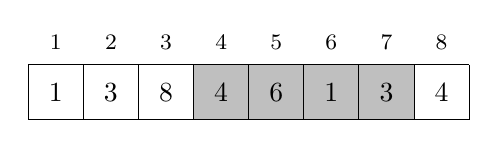
\begin{tikzpicture}[scale=0.7]
\fill[color=lightgray] (3,0) rectangle (7,1);
\draw (0,0) grid (8,1);

\node at (0.5,0.5) {$1$};
\node at (1.5,0.5) {$3$};
\node at (2.5,0.5) {$8$};
\node at (3.5,0.5) {$4$};
\node at (4.5,0.5) {$6$};
\node at (5.5,0.5) {$1$};
\node at (6.5,0.5) {$3$};
\node at (7.5,0.5) {$4$};

\footnotesize
\node at (0.5,1.4) {$1$};
\node at (1.5,1.4) {$2$};
\node at (2.5,1.4) {$3$};
\node at (3.5,1.4) {$4$};
\node at (4.5,1.4) {$5$};
\node at (5.5,1.4) {$6$};
\node at (6.5,1.4) {$7$};
\node at (7.5,1.4) {$8$};
\end{tikzpicture}
\end{center}

Helppo tapa vastata välikyselyyn on
käydä läpi kaikki välin alkiot silmukalla.
Esimerkiksi seuraava funktio toteuttaa summakyselyn:

\begin{lstlisting}
int summa(int a, int b) {
    int s = 0;
    for (int i = a; i <= b; i++) {
        s += t[i];
    }
    return s;
}
\end{lstlisting}

Yllä oleva funktio toteuttaa summakyselyn
ajassa $O(n)$, mikä on hidasta,
jos taulukko on suuri ja kyselyitä tulee paljon.
Tässä luvussa opimme, miten välikyselyitä pystyy
toteuttamaan huomattavasti nopeammin.

\section{Staattisen taulukon kyselyt}

Aloitamme yksinkertaisesta
tilanteesta, jossa taulukko on \key{staattinen}
eli sen sisältö ei muutu kyselyiden välillä.
Tällöin riittää muodostaa ennen kyselyitä
taulukon pohjalta tietorakenne,
josta voi selvittää tehokkaasti vastauksen mihin tahansa väliin
kohdistuvaan kyselyyn.

\subsubsection{Summakysely}

\index{summataulukko@summataulukko}

Summakyselyyn on mahdollista vastata tehokkaasti
muodostamalla taulukosta etukäteen \key{summataulukko},
jonka kohdassa $k$ on taulukon välin $[1,k]$ summa.
Tämän jälkeen minkä tahansa välin $[a,b]$
summan saa laskettua $O(1)$-ajassa
summataulukkoa käyttäen.

Esimerkiksi taulukon
\begin{center}
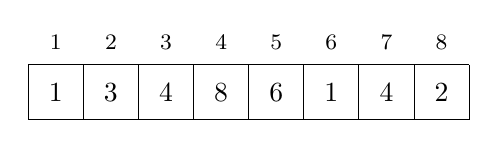
\begin{tikzpicture}[scale=0.7]
%\fill[color=lightgray] (3,0) rectangle (7,1);
\draw (0,0) grid (8,1);

\node at (0.5,0.5) {$1$};
\node at (1.5,0.5) {$3$};
\node at (2.5,0.5) {$4$};
\node at (3.5,0.5) {$8$};
\node at (4.5,0.5) {$6$};
\node at (5.5,0.5) {$1$};
\node at (6.5,0.5) {$4$};
\node at (7.5,0.5) {$2$};

\footnotesize
\node at (0.5,1.4) {$1$};
\node at (1.5,1.4) {$2$};
\node at (2.5,1.4) {$3$};
\node at (3.5,1.4) {$4$};
\node at (4.5,1.4) {$5$};
\node at (5.5,1.4) {$6$};
\node at (6.5,1.4) {$7$};
\node at (7.5,1.4) {$8$};
\end{tikzpicture}
\end{center}
summataulukko on seuraava:
\begin{center}
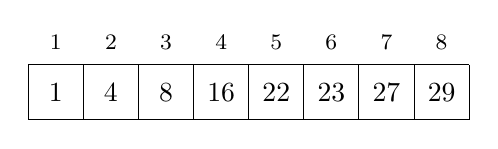
\begin{tikzpicture}[scale=0.7]
%\fill[color=lightgray] (3,0) rectangle (7,1);
\draw (0,0) grid (8,1);

\node at (0.5,0.5) {$1$};
\node at (1.5,0.5) {$4$};
\node at (2.5,0.5) {$8$};
\node at (3.5,0.5) {$16$};
\node at (4.5,0.5) {$22$};
\node at (5.5,0.5) {$23$};
\node at (6.5,0.5) {$27$};
\node at (7.5,0.5) {$29$};


\footnotesize
\node at (0.5,1.4) {$1$};
\node at (1.5,1.4) {$2$};
\node at (2.5,1.4) {$3$};
\node at (3.5,1.4) {$4$};
\node at (4.5,1.4) {$5$};
\node at (5.5,1.4) {$6$};
\node at (6.5,1.4) {$7$};
\node at (7.5,1.4) {$8$};
\end{tikzpicture}
\end{center}

Seuraava koodi muodostaa taulukosta \texttt{t}
summataulukon \texttt{s} ajassa $O(n)$:
\begin{lstlisting}
for (int i = 1; i <= n; i++) {
    s[i] = s[i-1]+t[i];
}
\end{lstlisting}
Tämän jälkeen summakyselyyn voi vastata
ajassa $O(1)$ seuraavasti:
\begin{lstlisting}
int summa(int a, int b) {
    return s[b]-s[a-1];
}
\end{lstlisting}

Funktio laskee välin $[a,b]$ summan
vähentämällä välin $[1,b]$ summasta
välin $[1,a-1]$ summan.
Summataulukosta riittää siis hakea kaksi arvoa
ja aikaa kuluu vain $O(1)$.
Huomaa, että 1-indeksoinnin ansiosta
funktio toimii myös tapauksessa $a=1$,
kunhan $\texttt{s}[0]=0$.

Tarkastellaan esimerkiksi väliä $[4,7]$:
\begin{center}
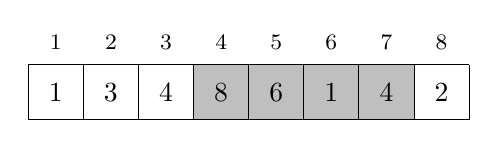
\begin{tikzpicture}[scale=0.7]
\fill[color=lightgray] (3,0) rectangle (7,1);
\draw (0,0) grid (8,1);

\node at (0.5,0.5) {$1$};
\node at (1.5,0.5) {$3$};
\node at (2.5,0.5) {$4$};
\node at (3.5,0.5) {$8$};
\node at (4.5,0.5) {$6$};
\node at (5.5,0.5) {$1$};
\node at (6.5,0.5) {$4$};
\node at (7.5,0.5) {$2$};

\footnotesize
\node at (0.5,1.4) {$1$};
\node at (1.5,1.4) {$2$};
\node at (2.5,1.4) {$3$};
\node at (3.5,1.4) {$4$};
\node at (4.5,1.4) {$5$};
\node at (5.5,1.4) {$6$};
\node at (6.5,1.4) {$7$};
\node at (7.5,1.4) {$8$};
\end{tikzpicture}
\end{center}
Välin $[4,7]$ summa on $8+6+1+4=19$.
Tämän saa laskettua tehokkaasti summataulukosta
etsimällä välien $[1,3]$ ja $[1,7]$ summat:
\begin{center}
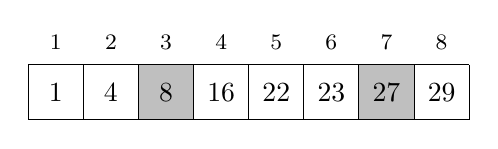
\begin{tikzpicture}[scale=0.7]
\fill[color=lightgray] (2,0) rectangle (3,1);
\fill[color=lightgray] (6,0) rectangle (7,1);
\draw (0,0) grid (8,1);

\node at (0.5,0.5) {$1$};
\node at (1.5,0.5) {$4$};
\node at (2.5,0.5) {$8$};
\node at (3.5,0.5) {$16$};
\node at (4.5,0.5) {$22$};
\node at (5.5,0.5) {$23$};
\node at (6.5,0.5) {$27$};
\node at (7.5,0.5) {$29$};


\footnotesize
\node at (0.5,1.4) {$1$};
\node at (1.5,1.4) {$2$};
\node at (2.5,1.4) {$3$};
\node at (3.5,1.4) {$4$};
\node at (4.5,1.4) {$5$};
\node at (5.5,1.4) {$6$};
\node at (6.5,1.4) {$7$};
\node at (7.5,1.4) {$8$};
\end{tikzpicture}
\end{center}
Välin $[4,7]$ summa on siis $27-8=19$.

Summataulukon idean voi yleistää
myös kaksiulotteiseen taulukkoon,
jolloin summataulukosta voi laskea
minkä tahansa suorakulmaisen alueen
summan $O(1)$-ajassa.
Tällöin summataulukkoon tallennetaan summia
alueista, jotka alkavat taulukon vasemmasta yläkulmasta.

\begin{samepage}
Seuraava ruudukko havainnollistaa asiaa:
\begin{center}
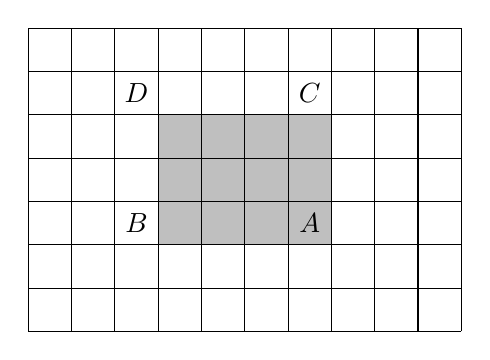
\begin{tikzpicture}[scale=0.55]
\draw[fill=lightgray] (3,2) rectangle (7,5);
\draw (0,0) grid (10,7);
%\draw[line width=2pt] (3,2) rectangle (7,5);
\node[anchor=center] at (6.5, 2.5) {$A$};
\node[anchor=center] at (2.5, 2.5) {$B$};
\node[anchor=center] at (6.5, 5.5) {$C$};
\node[anchor=center] at (2.5, 5.5) {$D$};
\end{tikzpicture}
\end{center}
\end{samepage}

Harmaan suorakulmion summan saa laskettua kaavalla
\[S(A) - S(B) - S(C) + S(D),\]
missä $S(X)$ tarkoittaa summaa vasemmasta
yläkulmasta kirjaimen $X$ osoittamaan kohtaan asti.

\subsubsection{Minimikysely}

Myös minimikyselyyn on mahdollista
vastata $O(1)$-ajassa sopivan esikäsittelyn avulla,
joskin tämä on vaikeampaa kuin summakyselyssä.
Huomaa, että minimikysely ja maksimikysely on
mahdollista toteuttaa aina samalla tavalla,
joten riittää keskittyä minimikyselyn toteutukseen. 

Ideana on laskea etukäteen taulukon jokaiselle
$2^k$-kokoiselle välille, mikä on kyseisen välin minimi.
Esimerkiksi taulukosta

\begin{center}
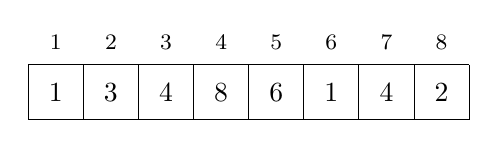
\begin{tikzpicture}[scale=0.7]
\draw (0,0) grid (8,1);

\node at (0.5,0.5) {$1$};
\node at (1.5,0.5) {$3$};
\node at (2.5,0.5) {$4$};
\node at (3.5,0.5) {$8$};
\node at (4.5,0.5) {$6$};
\node at (5.5,0.5) {$1$};
\node at (6.5,0.5) {$4$};
\node at (7.5,0.5) {$2$};

\footnotesize
\node at (0.5,1.4) {$1$};
\node at (1.5,1.4) {$2$};
\node at (2.5,1.4) {$3$};
\node at (3.5,1.4) {$4$};
\node at (4.5,1.4) {$5$};
\node at (5.5,1.4) {$6$};
\node at (6.5,1.4) {$7$};
\node at (7.5,1.4) {$8$};
\end{tikzpicture}
\end{center}
lasketaan seuraavat minimit:

\begin{center}
\begin{tabular}{ccc}

\begin{tabular}{ccc}
väli & koko & minimi \\
\hline
$[1,1]$ & 1 & 1 \\
$[2,2]$ & 1 & 3 \\
$[3,3]$ & 1 & 4 \\
$[4,4]$ & 1 & 8 \\
$[5,5]$ & 1 & 6 \\
$[6,6]$ & 1 & 1 \\
$[7,7]$ & 1 & 4 \\
$[8,8]$ & 1 & 2 \\
\end{tabular}

&

\begin{tabular}{ccc}
väli & koko & minimi \\
\hline
$[1,2]$ & 2 & 1 \\
$[2,3]$ & 2 & 3 \\
$[3,4]$ & 2 & 4 \\
$[4,5]$ & 2 & 6 \\
$[5,6]$ & 2 & 1 \\
$[6,7]$ & 2 & 1 \\
$[7,8]$ & 2 & 2 \\
\\
\end{tabular}

&

\begin{tabular}{ccc}
väli & koko & minimi \\
\hline
$[1,4]$ & 4 & 1 \\
$[2,5]$ & 4 & 3 \\
$[3,6]$ & 4 & 1 \\
$[4,7]$ & 4 & 1 \\
$[5,8]$ & 4 & 1 \\
$[1,8]$ & 8 & 1 \\
\\
\\
\end{tabular}

\end{tabular}

\end{center}

Taulukon $2^k$-välien määrä on $O(n \log n)$,
koska jokaisesta taulukon kohdasta alkaa
$O(\log n)$ väliä.
Kaikkien $2^k$-välien minimit pystytään laskemaan
ajassa $O(n \log n)$, koska jokainen $2^k$-väli
muodostuu kahdesta $2^{k-1}$ välistä ja
$2^k$-välin minimi on pienempi $2^{k-1}$-välien minimeistä.

Tämän jälkeen minkä tahansa välin $[a,b]$ minimin
saa laskettua $O(1)$-ajassa miniminä kahdesta $2^k$-välistä,
missä $k=\lfloor \log_2(b-a+1) \rfloor$.
Ensimmäinen väli alkaa kohdasta $a$
ja toinen väli päättyy kohtaan $b$.
Parametri $k$ on valittu niin,
että kaksi $2^k$-kokoista väliä
kattaa koko välin $[a,b]$.

Tarkastellaan esimerkiksi väliä $[2,7]$:
\begin{center}
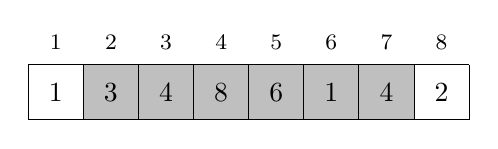
\begin{tikzpicture}[scale=0.7]
\fill[color=lightgray] (1,0) rectangle (7,1);
\draw (0,0) grid (8,1);

\node at (0.5,0.5) {$1$};
\node at (1.5,0.5) {$3$};
\node at (2.5,0.5) {$4$};
\node at (3.5,0.5) {$8$};
\node at (4.5,0.5) {$6$};
\node at (5.5,0.5) {$1$};
\node at (6.5,0.5) {$4$};
\node at (7.5,0.5) {$2$};

\footnotesize
\node at (0.5,1.4) {$1$};
\node at (1.5,1.4) {$2$};
\node at (2.5,1.4) {$3$};
\node at (3.5,1.4) {$4$};
\node at (4.5,1.4) {$5$};
\node at (5.5,1.4) {$6$};
\node at (6.5,1.4) {$7$};
\node at (7.5,1.4) {$8$};
\end{tikzpicture}
\end{center}
Välin $[2,7]$ pituus on 6 ja $\lfloor \log_2(6) \rfloor = 2$.
Niinpä välin minimin saa selville kahden 4-pituisen
välin minimistä.
Välit ovat $[2,5]$ ja $[4,7]$:
\begin{center}
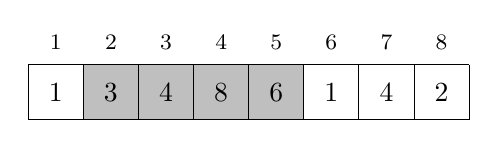
\begin{tikzpicture}[scale=0.7]
\fill[color=lightgray] (1,0) rectangle (5,1);
\draw (0,0) grid (8,1);

\node at (0.5,0.5) {$1$};
\node at (1.5,0.5) {$3$};
\node at (2.5,0.5) {$4$};
\node at (3.5,0.5) {$8$};
\node at (4.5,0.5) {$6$};
\node at (5.5,0.5) {$1$};
\node at (6.5,0.5) {$4$};
\node at (7.5,0.5) {$2$};

\footnotesize
\node at (0.5,1.4) {$1$};
\node at (1.5,1.4) {$2$};
\node at (2.5,1.4) {$3$};
\node at (3.5,1.4) {$4$};
\node at (4.5,1.4) {$5$};
\node at (5.5,1.4) {$6$};
\node at (6.5,1.4) {$7$};
\node at (7.5,1.4) {$8$};
\end{tikzpicture}
\end{center}
\begin{center}
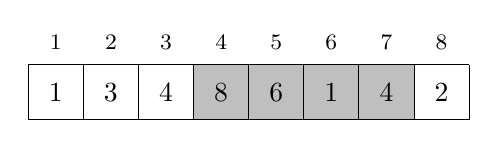
\begin{tikzpicture}[scale=0.7]
\fill[color=lightgray] (3,0) rectangle (7,1);
\draw (0,0) grid (8,1);

\node at (0.5,0.5) {$1$};
\node at (1.5,0.5) {$3$};
\node at (2.5,0.5) {$4$};
\node at (3.5,0.5) {$8$};
\node at (4.5,0.5) {$6$};
\node at (5.5,0.5) {$1$};
\node at (6.5,0.5) {$4$};
\node at (7.5,0.5) {$2$};


\footnotesize
\node at (0.5,1.4) {$1$};
\node at (1.5,1.4) {$2$};
\node at (2.5,1.4) {$3$};
\node at (3.5,1.4) {$4$};
\node at (4.5,1.4) {$5$};
\node at (5.5,1.4) {$6$};
\node at (6.5,1.4) {$7$};
\node at (7.5,1.4) {$8$};
\end{tikzpicture}
\end{center}
Välin $[2,5]$ minimi on 3 ja välin $[4,7]$ minimi on 1.
Tämän seurauksena välin $[2,7]$ minimi on pienempi näistä eli 1.
% 
% Mainittakoon, että $O(1)$-aikaiset minimikyselyt pystyy
% toteuttamaan myös niin, että esikäsittely vie aikaa
% vain $O(n)$ eikä $O(n \log n)$.
% Tämä on kuitenkin selvästi vaikeampaa, eikä 
% sillä ole merkitystä kisakoodauksessa.

\section{Binääri-indeksipuu}

\index{binxxri-indeksipuu@binääri-indeksipuu}
\index{Fenwick-puu}

\key{Binääri-indeksipuu} eli \key{Fenwick-puu} on
summataulukkoa muistuttava tietorakenne,
joka toteuttaa kaksi operaatiota:
taulukon välin $[a,b]$ summakysely
sekä taulukon kohdassa $k$ olevan luvun päivitys.
Kummankin operaation aikavaativuus on $O(\log n)$.

Binääri-indeksipuun etuna summataulukkoon verrattuna on,
että taulukkoa pystyy päivittämään tehokkaasti
summakyselyiden välissä.
Summataulukossa tämä ei olisi mahdollista,
vaan koko summataulukko tulisi muodostaa uudestaan $O(n)$-ajassa
taulukon päivityksen jälkeen.

\subsubsection{Rakenne}

Binääri-indeksipuu on taulukko, jonka
kohdassa $k$ on kohtaan $k$ päättyvän välin lukujen summa
alkuperäisessä taulukossa.
Välin pituus on suurin 2:n potenssi, jolla $k$ on jaollinen.
Esimerkiksi jos $k=6$, välin pituus on 2, koska
6 on jaollinen 2:lla mutta ei ole jaollinen 4:llä.

\begin{samepage}
Esimerkiksi taulukkoa
\begin{center}
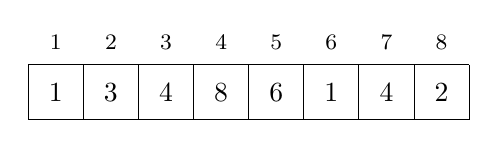
\begin{tikzpicture}[scale=0.7]
\draw (0,0) grid (8,1);

\node at (0.5,0.5) {$1$};
\node at (1.5,0.5) {$3$};
\node at (2.5,0.5) {$4$};
\node at (3.5,0.5) {$8$};
\node at (4.5,0.5) {$6$};
\node at (5.5,0.5) {$1$};
\node at (6.5,0.5) {$4$};
\node at (7.5,0.5) {$2$};

\footnotesize
\node at (0.5,1.4) {$1$};
\node at (1.5,1.4) {$2$};
\node at (2.5,1.4) {$3$};
\node at (3.5,1.4) {$4$};
\node at (4.5,1.4) {$5$};
\node at (5.5,1.4) {$6$};
\node at (6.5,1.4) {$7$};
\node at (7.5,1.4) {$8$};
\end{tikzpicture}
\end{center}
\end{samepage}
vastaava binääri-indeksipuu on seuraava:
\begin{center}
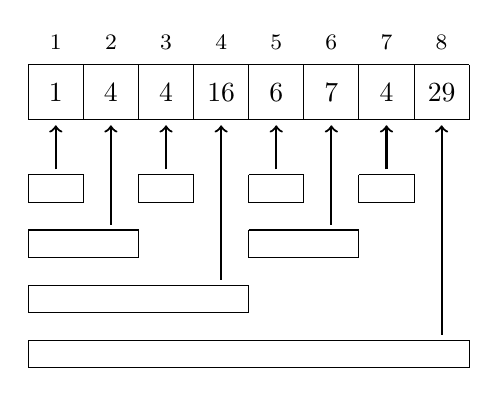
\begin{tikzpicture}[scale=0.7]
%\fill[color=lightgray] (3,0) rectangle (7,1);
\draw (0,0) grid (8,1);

\node at (0.5,0.5) {$1$};
\node at (1.5,0.5) {$4$};
\node at (2.5,0.5) {$4$};
\node at (3.5,0.5) {$16$};
\node at (4.5,0.5) {$6$};
\node at (5.5,0.5) {$7$};
\node at (6.5,0.5) {$4$};
\node at (7.5,0.5) {$29$};

\footnotesize
\node at (0.5,1.4) {$1$};
\node at (1.5,1.4) {$2$};
\node at (2.5,1.4) {$3$};
\node at (3.5,1.4) {$4$};
\node at (4.5,1.4) {$5$};
\node at (5.5,1.4) {$6$};
\node at (6.5,1.4) {$7$};
\node at (7.5,1.4) {$8$};

\draw[->,thick] (0.5,-0.9) -- (0.5,-0.1);
\draw[->,thick] (2.5,-0.9) -- (2.5,-0.1);
\draw[->,thick] (4.5,-0.9) -- (4.5,-0.1);
\draw[->,thick] (6.5,-0.9) -- (6.5,-0.1);
\draw[->,thick] (1.5,-1.9) -- (1.5,-0.1);
\draw[->,thick] (5.5,-1.9) -- (5.5,-0.1);
\draw[->,thick] (3.5,-2.9) -- (3.5,-0.1);
\draw[->,thick] (7.5,-3.9) -- (7.5,-0.1);

\draw (0,-1) -- (1,-1) -- (1,-1.5) -- (0,-1.5) -- (0,-1);
\draw (2,-1) -- (3,-1) -- (3,-1.5) -- (2,-1.5) -- (2,-1);
\draw (4,-1) -- (5,-1) -- (5,-1.5) -- (4,-1.5) -- (4,-1);
\draw (6,-1) -- (7,-1) -- (7,-1.5) -- (6,-1.5) -- (6,-1);
\draw (0,-2) -- (2,-2) -- (2,-2.5) -- (0,-2.5) -- (0,-2);
\draw (4,-2) -- (6,-2) -- (6,-2.5) -- (4,-2.5) -- (4,-2);
\draw (0,-3) -- (4,-3) -- (4,-3.5) -- (0,-3.5) -- (0,-3);
\draw (0,-4) -- (8,-4) -- (8,-4.5) -- (0,-4.5) -- (0,-4);
\end{tikzpicture}
\end{center}

Esimerkiksi binääri-indeksipuun kohdassa 6 on luku 7,
koska välin $[5,6]$ lukujen summa on $6+1=7$.

\subsubsection{Summakysely}

Binääri-indeksipuun perusoperaatio on välin $[1,k]$
summan laskeminen, missä $k$ on mikä tahansa taulukon kohta.
Tällaisen summan pystyy muodostamaan aina laskemalla yhteen
puussa olevia välien summia.

Esimerkiksi välin $[1,7]$
summa muodostuu seuraavista summista:
\begin{center}
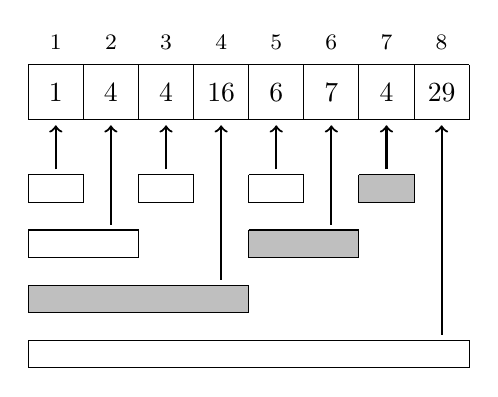
\begin{tikzpicture}[scale=0.7]
%\fill[color=lightgray] (3,0) rectangle (7,1);
\draw (0,0) grid (8,1);

\node at (0.5,0.5) {$1$};
\node at (1.5,0.5) {$4$};
\node at (2.5,0.5) {$4$};
\node at (3.5,0.5) {$16$};
\node at (4.5,0.5) {$6$};
\node at (5.5,0.5) {$7$};
\node at (6.5,0.5) {$4$};
\node at (7.5,0.5) {$29$};

\footnotesize
\node at (0.5,1.4) {$1$};
\node at (1.5,1.4) {$2$};
\node at (2.5,1.4) {$3$};
\node at (3.5,1.4) {$4$};
\node at (4.5,1.4) {$5$};
\node at (5.5,1.4) {$6$};
\node at (6.5,1.4) {$7$};
\node at (7.5,1.4) {$8$};

\draw[->,thick] (0.5,-0.9) -- (0.5,-0.1);
\draw[->,thick] (2.5,-0.9) -- (2.5,-0.1);
\draw[->,thick] (4.5,-0.9) -- (4.5,-0.1);
\draw[->,thick] (6.5,-0.9) -- (6.5,-0.1);
\draw[->,thick] (1.5,-1.9) -- (1.5,-0.1);
\draw[->,thick] (5.5,-1.9) -- (5.5,-0.1);
\draw[->,thick] (3.5,-2.9) -- (3.5,-0.1);
\draw[->,thick] (7.5,-3.9) -- (7.5,-0.1);

\draw (0,-1) -- (1,-1) -- (1,-1.5) -- (0,-1.5) -- (0,-1);
\draw (2,-1) -- (3,-1) -- (3,-1.5) -- (2,-1.5) -- (2,-1);
\draw (4,-1) -- (5,-1) -- (5,-1.5) -- (4,-1.5) -- (4,-1);
\draw[fill=lightgray] (6,-1) -- (7,-1) -- (7,-1.5) -- (6,-1.5) -- (6,-1);
\draw (0,-2) -- (2,-2) -- (2,-2.5) -- (0,-2.5) -- (0,-2);
\draw[fill=lightgray] (4,-2) -- (6,-2) -- (6,-2.5) -- (4,-2.5) -- (4,-2);
\draw[fill=lightgray] (0,-3) -- (4,-3) -- (4,-3.5) -- (0,-3.5) -- (0,-3);
\draw (0,-4) -- (8,-4) -- (8,-4.5) -- (0,-4.5) -- (0,-4);
\end{tikzpicture}
\end{center}

Välin $[1,7]$ summa on siis $16+7+4=27$.
Binääri-indeksipuun rakenteen ansiosta
jokainen summaan kuuluva väli on eripituinen.
Niinpä summa muodostuu aina $O(\log n)$ välin summasta.

Summataulukon tavoin binääri-indeksipuusta voi laskea
tehokkaasti minkä tahansa taulukon välin summan,
koska välin $[a,b]$ summa saadaan vähentämällä
välin $[1,b]$ summasta välin $[1,a-1]$ summa.
Aikavaativuus on edelleen $O(\log n)$,
koska riittää laskea kaksi $[1,k]$-välin summaa.

\subsubsection{Taulukon päivitys}

Kun taulukon kohdassa $k$ oleva luku muuttuu,
tämä vaikuttaa useaan
binääri-indeksi\-puussa olevaan summaan.
Esimerkiksi jos kohdassa 3 oleva luku muuttuu,
seuraavat välien summat muuttuvat:
\begin{center}
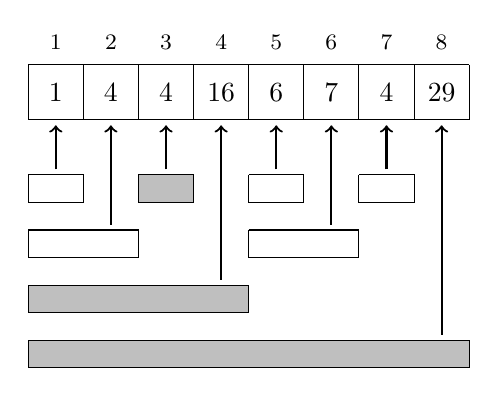
\begin{tikzpicture}[scale=0.7]
%\fill[color=lightgray] (3,0) rectangle (7,1);
\draw (0,0) grid (8,1);

\node at (0.5,0.5) {$1$};
\node at (1.5,0.5) {$4$};
\node at (2.5,0.5) {$4$};
\node at (3.5,0.5) {$16$};
\node at (4.5,0.5) {$6$};
\node at (5.5,0.5) {$7$};
\node at (6.5,0.5) {$4$};
\node at (7.5,0.5) {$29$};

\footnotesize
\node at (0.5,1.4) {$1$};
\node at (1.5,1.4) {$2$};
\node at (2.5,1.4) {$3$};
\node at (3.5,1.4) {$4$};
\node at (4.5,1.4) {$5$};
\node at (5.5,1.4) {$6$};
\node at (6.5,1.4) {$7$};
\node at (7.5,1.4) {$8$};

\draw[->,thick] (0.5,-0.9) -- (0.5,-0.1);
\draw[->,thick] (2.5,-0.9) -- (2.5,-0.1);
\draw[->,thick] (4.5,-0.9) -- (4.5,-0.1);
\draw[->,thick] (6.5,-0.9) -- (6.5,-0.1);
\draw[->,thick] (1.5,-1.9) -- (1.5,-0.1);
\draw[->,thick] (5.5,-1.9) -- (5.5,-0.1);
\draw[->,thick] (3.5,-2.9) -- (3.5,-0.1);
\draw[->,thick] (7.5,-3.9) -- (7.5,-0.1);

\draw (0,-1) -- (1,-1) -- (1,-1.5) -- (0,-1.5) -- (0,-1);
\draw[fill=lightgray] (2,-1) -- (3,-1) -- (3,-1.5) -- (2,-1.5) -- (2,-1);
\draw (4,-1) -- (5,-1) -- (5,-1.5) -- (4,-1.5) -- (4,-1);
\draw (6,-1) -- (7,-1) -- (7,-1.5) -- (6,-1.5) -- (6,-1);
\draw (0,-2) -- (2,-2) -- (2,-2.5) -- (0,-2.5) -- (0,-2);
\draw (4,-2) -- (6,-2) -- (6,-2.5) -- (4,-2.5) -- (4,-2);
\draw[fill=lightgray] (0,-3) -- (4,-3) -- (4,-3.5) -- (0,-3.5) -- (0,-3);
\draw[fill=lightgray] (0,-4) -- (8,-4) -- (8,-4.5) -- (0,-4.5) -- (0,-4);
\end{tikzpicture}
\end{center}

Myös tässä tapauksessa kaikki välit,
joihin muutos vaikuttaa, ovat eripituisia,
joten muutos kohdistuu $O(\log n)$ kohtaan
binääri-indeksipuussa.

\subsubsection{Toteutus}

Binääri-indeksipuun operaatiot on mahdollista toteuttaa 
lyhyesti ja tehokkaasti bittien käsittelyn avulla.
Oleellinen bittioperaatio on $k \& -k$,
joka eristää luvusta $k$ viimeisenä olevan ykkösbitin.
Esimerkiksi $6 \& -6=2$, koska luku $6$ on bittimuodossa 110
ja luku $2$ on bittimuodossa on 10.

Osoittautuu, että summan laskemisessa
binääri-indeksipuun kohtaa $k$ tulee muuttaa joka askeleella niin,
että siitä poistetaan luku $k \& -k$.
Vastaavasti taulukon päivityksessä kohtaa $k$ tulee muuttaa joka askeleella niin,
että siihen lisätään luku $k \& -k$.


Seuraavat funktiot olettavat, että binääri-indeksipuu on
tallennettu taulukkoon \texttt{b} ja se muodostuu kohdista $1 \ldots n$.

Funktio \texttt{summa} laskee välin $[1,k]$ summan:
\begin{lstlisting}
int summa(int k) {
    int s = 0;
    while (k >= 1) {
        s += b[k];
        k -= k&-k;
    }
    return s;
}
\end{lstlisting}

Funktio \texttt{lisaa} kasvattaa taulukon kohtaa $k$ arvolla $x$:
\begin{lstlisting}
void lisaa(int k, int x) {
    while (k <= n) {
        b[k] += x;
        k += k&-k;
    }
}
\end{lstlisting}

Kummankin yllä olevan funktion aikavaativuus on $O(\log n)$,
koska funktiot muuttavat $O(\log n)$ kohtaa
binääri-indeksipuussa ja uuteen kohtaan siirtyminen
vie aikaa $O(1)$ bittioperaation avulla.

\section{Segmenttipuu}

\index{segmenttipuu@segmenttipuu}

\key{Segmenttipuu} on tietorakenne,
jonka operaatiot ovat taulukon välin $[a,b]$ välikysely
sekä kohdan $k$ arvon päivitys.
Segmenttipuun avulla voi toteuttaa summakyselyn,
minimikyselyn ja monia muitakin kyselyitä niin,
että kummankin operaation aikavaativuus on $O(\log n)$.

Segmenttipuun etuna binääri-indeksipuuhun verrattuna on,
että se on yleisempi tietorakenne.
Binääri-indeksipuulla voi toteuttaa vain summakyselyn,
mutta segmenttipuu sallii muitakin kyselyitä.
Toisaalta segmenttipuu vie enemmän muistia ja
on hieman vaikeampi toteuttaa kuin binääri-indeksipuu.

\subsubsection{Rakenne}

Segmenttipuussa on $2n-1$ solmua niin,
että alimmalla tasolla on $n$ solmua,
jotka kuvaavat taulukon sisällön,
ja ylemmillä tasoilla on välikyselyihin
tarvittavaa tietoa.
Segmenttipuun sisältö riippuu siitä,
mikä välikysely puun tulee toteuttaa.
Oletamme aluksi, että välikysely on tuttu summakysely.

Esimerkiksi taulukkoa
\begin{center}
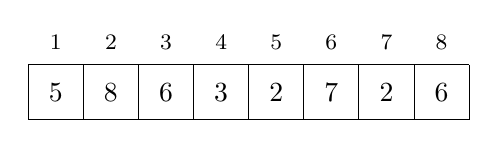
\begin{tikzpicture}[scale=0.7]
\draw (0,0) grid (8,1);

\node at (0.5,0.5) {$5$};
\node at (1.5,0.5) {$8$};
\node at (2.5,0.5) {$6$};
\node at (3.5,0.5) {$3$};
\node at (4.5,0.5) {$2$};
\node at (5.5,0.5) {$7$};
\node at (6.5,0.5) {$2$};
\node at (7.5,0.5) {$6$};

\footnotesize
\node at (0.5,1.4) {$1$};
\node at (1.5,1.4) {$2$};
\node at (2.5,1.4) {$3$};
\node at (3.5,1.4) {$4$};
\node at (4.5,1.4) {$5$};
\node at (5.5,1.4) {$6$};
\node at (6.5,1.4) {$7$};
\node at (7.5,1.4) {$8$};
\end{tikzpicture}
\end{center}
vastaa seuraava segmenttipuu:
\begin{center}
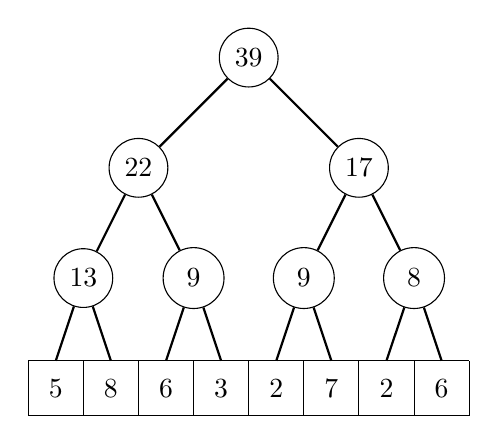
\begin{tikzpicture}[scale=0.7]
\draw (0,0) grid (8,1);

\node[anchor=center] at (0.5, 0.5) {5};
\node[anchor=center] at (1.5, 0.5) {8};
\node[anchor=center] at (2.5, 0.5) {6};
\node[anchor=center] at (3.5, 0.5) {3};
\node[anchor=center] at (4.5, 0.5) {2};
\node[anchor=center] at (5.5, 0.5) {7};
\node[anchor=center] at (6.5, 0.5) {2};
\node[anchor=center] at (7.5, 0.5) {6};

\node[draw, circle] (a) at (1,2.5) {13};
\path[draw,thick,-] (a) -- (0.5,1);
\path[draw,thick,-] (a) -- (1.5,1);
\node[draw, circle,minimum size=22pt] (b) at (3,2.5) {9};
\path[draw,thick,-] (b) -- (2.5,1);
\path[draw,thick,-] (b) -- (3.5,1);
\node[draw, circle,minimum size=22pt] (c) at (5,2.5) {9};
\path[draw,thick,-] (c) -- (4.5,1);
\path[draw,thick,-] (c) -- (5.5,1);
\node[draw, circle,minimum size=22pt] (d) at (7,2.5) {8};
\path[draw,thick,-] (d) -- (6.5,1);
\path[draw,thick,-] (d) -- (7.5,1);

\node[draw, circle] (i) at (2,4.5) {22};
\path[draw,thick,-] (i) -- (a);
\path[draw,thick,-] (i) -- (b);
\node[draw, circle] (j) at (6,4.5) {17};
\path[draw,thick,-] (j) -- (c);
\path[draw,thick,-] (j) -- (d);

\node[draw, circle] (m) at (4,6.5) {39};
\path[draw,thick,-] (m) -- (i);
\path[draw,thick,-] (m) -- (j);
\end{tikzpicture}
\end{center}

Jokaisessa segmenttipuun solmussa on tietoa
$2^k$-kokoisesta välistä taulukossa.
Tässä tapauksessa solmussa oleva arvo kertoo,
mikä on taulukon lukujen summa solmua vastaavalla
välillä.
Kunkin solmun arvo saadaan laskemalla yhteen
solmun alapuolella vasemmalla ja oikealla
olevien solmujen arvot.

Segmenttipuu on mukavinta rakentaa niin,
että taulukon koko on 2:n potenssi,
jolloin tuloksena on täydellinen binääripuu.
Jatkossa oletamme aina,
että taulukko täyttää tämän vaatimuksen.
Jos taulukon koko ei ole 2:n potenssi,
sen loppuun voi lisätä tyhjää niin,
että koosta tulee 2:n potenssi.

\subsubsection{Välikysely}

Segmenttipuussa vastaus välikyselyyn lasketaan
väliin kuuluvista solmuista,
jotka ovat mahdollisimman korkealla puussa.
Jokainen solmu antaa vastauksen väliin kuuluvalle osavälille,
ja vastaus kyselyyn selviää yhdistämällä
segmenttipuusta saadut osavälejä koskeva tiedot.

Tarkastellaan esimerkiksi seuraavaa taulukon väliä:
\begin{center}
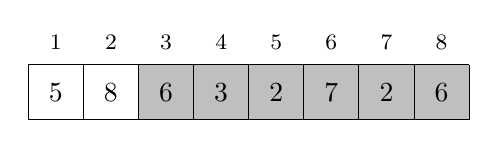
\begin{tikzpicture}[scale=0.7]
\fill[color=gray!50] (2,0) rectangle (8,1);
\draw (0,0) grid (8,1);

\node[anchor=center] at (0.5, 0.5) {5};
\node[anchor=center] at (1.5, 0.5) {8};
\node[anchor=center] at (2.5, 0.5) {6};
\node[anchor=center] at (3.5, 0.5) {3};
\node[anchor=center] at (4.5, 0.5) {2};
\node[anchor=center] at (5.5, 0.5) {7};
\node[anchor=center] at (6.5, 0.5) {2};
\node[anchor=center] at (7.5, 0.5) {6};

\footnotesize
\node at (0.5,1.4) {$1$};
\node at (1.5,1.4) {$2$};
\node at (2.5,1.4) {$3$};
\node at (3.5,1.4) {$4$};
\node at (4.5,1.4) {$5$};
\node at (5.5,1.4) {$6$};
\node at (6.5,1.4) {$7$};
\node at (7.5,1.4) {$8$};
\end{tikzpicture}
\end{center}
Lukujen summa välillä $[3,8]$ on $6+3+2+7+2+6=26$.
Segmenttipuusta summa saadaan laskettua seuraavien
osasummien avulla:
\begin{center}
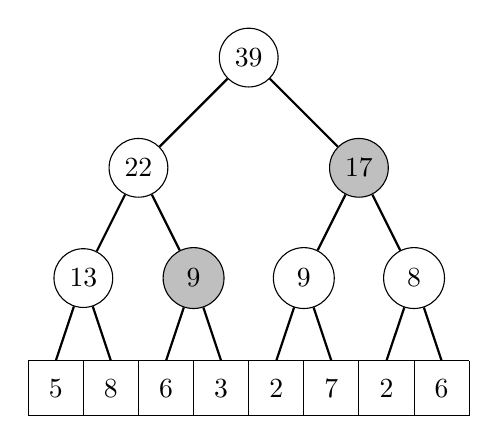
\begin{tikzpicture}[scale=0.7]
\draw (0,0) grid (8,1);

\node[anchor=center] at (0.5, 0.5) {5};
\node[anchor=center] at (1.5, 0.5) {8};
\node[anchor=center] at (2.5, 0.5) {6};
\node[anchor=center] at (3.5, 0.5) {3};
\node[anchor=center] at (4.5, 0.5) {2};
\node[anchor=center] at (5.5, 0.5) {7};
\node[anchor=center] at (6.5, 0.5) {2};
\node[anchor=center] at (7.5, 0.5) {6};

\node[draw, circle] (a) at (1,2.5) {13};
\path[draw,thick,-] (a) -- (0.5,1);
\path[draw,thick,-] (a) -- (1.5,1);
\node[draw, circle,fill=gray!50,minimum size=22pt] (b) at (3,2.5) {9};
\path[draw,thick,-] (b) -- (2.5,1);
\path[draw,thick,-] (b) -- (3.5,1);
\node[draw, circle,minimum size=22pt] (c) at (5,2.5) {9};
\path[draw,thick,-] (c) -- (4.5,1);
\path[draw,thick,-] (c) -- (5.5,1);
\node[draw, circle,minimum size=22pt] (d) at (7,2.5) {8};
\path[draw,thick,-] (d) -- (6.5,1);
\path[draw,thick,-] (d) -- (7.5,1);

\node[draw, circle] (i) at (2,4.5) {22};
\path[draw,thick,-] (i) -- (a);
\path[draw,thick,-] (i) -- (b);
\node[draw, circle,fill=gray!50] (j) at (6,4.5) {17};
\path[draw,thick,-] (j) -- (c);
\path[draw,thick,-] (j) -- (d);

\node[draw, circle] (m) at (4,6.5) {39};
\path[draw,thick,-] (m) -- (i);
\path[draw,thick,-] (m) -- (j);
\end{tikzpicture}
\end{center}
Taulukon välin summaksi tulee osasummista $9+17=26$.

Kun vastaus välikyselyyn lasketaan mahdollisimman
korkealla segmenttipuussa olevista solmuista,
väliin kuuluu enintään kaksi solmua
jokaiselta segmenttipuun tasolta.
Tämän ansiosta välikyselyssä
tarvittavien solmujen yhteismäärä on vain $O(\log n)$.

\subsubsection{Taulukon päivitys}

Kun taulukossa oleva arvo muuttuu,
segmenttipuussa täytyy päivittää
kaikkia solmuja, joiden arvo
riippuu muutetusta taulukon kohdasta.
Tämä tapahtuu kulkemalla puuta ylöspäin huipulle
asti ja tekemällä muutokset.

\begin{samepage}
Seuraava kuva näyttää, mitkä solmut segmenttipuussa muuttuvat,
jos taulukon luku 7 muuttuu.

\begin{center}
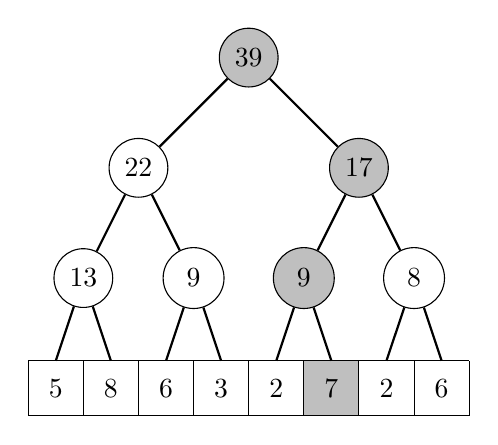
\begin{tikzpicture}[scale=0.7]
\fill[color=gray!50] (5,0) rectangle (6,1);
\draw (0,0) grid (8,1);

\node[anchor=center] at (0.5, 0.5) {5};
\node[anchor=center] at (1.5, 0.5) {8};
\node[anchor=center] at (2.5, 0.5) {6};
\node[anchor=center] at (3.5, 0.5) {3};
\node[anchor=center] at (4.5, 0.5) {2};
\node[anchor=center] at (5.5, 0.5) {7};
\node[anchor=center] at (6.5, 0.5) {2};
\node[anchor=center] at (7.5, 0.5) {6};

\node[draw, circle] (a) at (1,2.5) {13};
\path[draw,thick,-] (a) -- (0.5,1);
\path[draw,thick,-] (a) -- (1.5,1);
\node[draw, circle,minimum size=22pt] (b) at (3,2.5) {9};
\path[draw,thick,-] (b) -- (2.5,1);
\path[draw,thick,-] (b) -- (3.5,1);
\node[draw, circle,minimum size=22pt,fill=gray!50] (c) at (5,2.5) {9};
\path[draw,thick,-] (c) -- (4.5,1);
\path[draw,thick,-] (c) -- (5.5,1);
\node[draw, circle,minimum size=22pt] (d) at (7,2.5) {8};
\path[draw,thick,-] (d) -- (6.5,1);
\path[draw,thick,-] (d) -- (7.5,1);

\node[draw, circle] (i) at (2,4.5) {22};
\path[draw,thick,-] (i) -- (a);
\path[draw,thick,-] (i) -- (b);
\node[draw, circle,fill=gray!50] (j) at (6,4.5) {17};
\path[draw,thick,-] (j) -- (c);
\path[draw,thick,-] (j) -- (d);

\node[draw, circle,fill=gray!50] (m) at (4,6.5) {39};
\path[draw,thick,-] (m) -- (i);
\path[draw,thick,-] (m) -- (j);
\end{tikzpicture}
\end{center}
\end{samepage}

Polku segmenttipuun pohjalta huipulle muodostuu aina $O(\log n)$ solmusta,
joten taulukon arvon muuttuminen vaikuttaa $O(\log n)$ solmuun puussa.

\subsubsection{Puun tallennus}

Segmenttipuun voi tallentaa muistiin 
$2N$ alkion taulukkona,
jossa $N$ on riittävän suuri 2:n potenssi.
Tällaisen segmenttipuun avulla voi ylläpitää
taulukkoa, jonka indeksialue on $[0,N-1]$.

Segmenttipuun taulukon
kohdassa 1 on puun ylimmän solmun arvo,
kohdat 2 ja 3 sisältävät seuraavan tason
solmujen arvot, jne.
Segmenttipuun alin taso eli varsinainen
taulukon sisältä tallennetaan
kohdasta $N$ alkaen.
Niinpä taulukon kohdassa $k$ oleva alkio
on segmenttipuun taulukossa kohdassa $k+N$.

Esimerkiksi segmenttipuun
\begin{center}
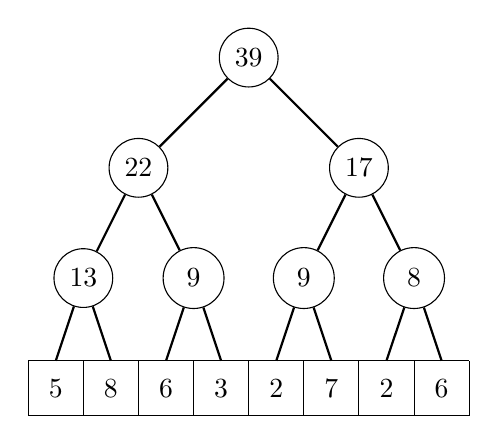
\begin{tikzpicture}[scale=0.7]
\draw (0,0) grid (8,1);

\node[anchor=center] at (0.5, 0.5) {5};
\node[anchor=center] at (1.5, 0.5) {8};
\node[anchor=center] at (2.5, 0.5) {6};
\node[anchor=center] at (3.5, 0.5) {3};
\node[anchor=center] at (4.5, 0.5) {2};
\node[anchor=center] at (5.5, 0.5) {7};
\node[anchor=center] at (6.5, 0.5) {2};
\node[anchor=center] at (7.5, 0.5) {6};

\node[draw, circle] (a) at (1,2.5) {13};
\path[draw,thick,-] (a) -- (0.5,1);
\path[draw,thick,-] (a) -- (1.5,1);
\node[draw, circle,minimum size=22pt] (b) at (3,2.5) {9};
\path[draw,thick,-] (b) -- (2.5,1);
\path[draw,thick,-] (b) -- (3.5,1);
\node[draw, circle,minimum size=22pt] (c) at (5,2.5) {9};
\path[draw,thick,-] (c) -- (4.5,1);
\path[draw,thick,-] (c) -- (5.5,1);
\node[draw, circle,minimum size=22pt] (d) at (7,2.5) {8};
\path[draw,thick,-] (d) -- (6.5,1);
\path[draw,thick,-] (d) -- (7.5,1);

\node[draw, circle] (i) at (2,4.5) {22};
\path[draw,thick,-] (i) -- (a);
\path[draw,thick,-] (i) -- (b);
\node[draw, circle] (j) at (6,4.5) {17};
\path[draw,thick,-] (j) -- (c);
\path[draw,thick,-] (j) -- (d);

\node[draw, circle] (m) at (4,6.5) {39};
\path[draw,thick,-] (m) -- (i);
\path[draw,thick,-] (m) -- (j);
\end{tikzpicture}
\end{center}
voi tallentaa taulukkoon seuraavasti ($N=8$):
\begin{center}
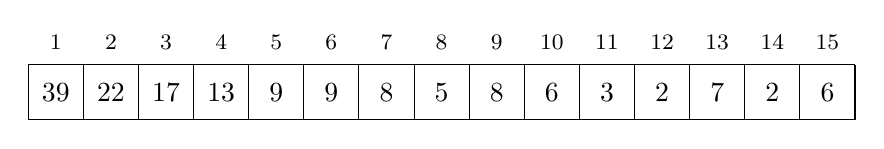
\begin{tikzpicture}[scale=0.7]
%\fill[color=lightgray] (3,0) rectangle (7,1);
\draw (0,0) grid (15,1);

\node at (0.5,0.5) {$39$};
\node at (1.5,0.5) {$22$};
\node at (2.5,0.5) {$17$};
\node at (3.5,0.5) {$13$};
\node at (4.5,0.5) {$9$};
\node at (5.5,0.5) {$9$};
\node at (6.5,0.5) {$8$};
\node at (7.5,0.5) {$5$};
\node at (8.5,0.5) {$8$};
\node at (9.5,0.5) {$6$};
\node at (10.5,0.5) {$3$};
\node at (11.5,0.5) {$2$};
\node at (12.5,0.5) {$7$};
\node at (13.5,0.5) {$2$};
\node at (14.5,0.5) {$6$};

\footnotesize
\node at (0.5,1.4) {$1$};
\node at (1.5,1.4) {$2$};
\node at (2.5,1.4) {$3$};
\node at (3.5,1.4) {$4$};
\node at (4.5,1.4) {$5$};
\node at (5.5,1.4) {$6$};
\node at (6.5,1.4) {$7$};
\node at (7.5,1.4) {$8$};
\node at (8.5,1.4) {$9$};
\node at (9.5,1.4) {$10$};
\node at (10.5,1.4) {$11$};
\node at (11.5,1.4) {$12$};
\node at (12.5,1.4) {$13$};
\node at (13.5,1.4) {$14$};
\node at (14.5,1.4) {$15$};
\end{tikzpicture}
\end{center}
Tätä tallennustapaa käyttäen kohdassa $k$
olevalle solmulle pätee, että
\begin{itemize}
\item ylempi solmu on kohdassa $\lfloor k/2 \rfloor$,
\item vasen alempi solmu on kohdassa $2k$ ja
\item oikea alempi solmu on kohdassa $2k+1$.
\end{itemize}
Huomaa, että tämän seurauksena solmun kohta on parillinen,
jos se on vasemmalla ylemmästä solmusta katsoen,
ja pariton, jos se on oikealla.

\subsubsection{Toteutus}

Tarkastellaan seuraavaksi välikyselyn ja päivityksen
toteutusta segmenttipuuhun.
Seuraavat funktiot olettavat, että segmenttipuu
on tallennettu $2n-1$-kokoi\-seen taulukkoon $\texttt{p}$
edellä kuvatulla tavalla.

Funktio \texttt{summa} laskee summan
välillä $a \ldots b$:

\begin{lstlisting}
int summa(int a, int b) {
    a += N; b += N;
    int s = 0;
    while (a <= b) {
        if (a%2 == 1) s += p[a++];
        if (b%2 == 0) s += p[b--];
        a /= 2; b /= 2;
    }
    return s;
}
\end{lstlisting}

Funktio aloittaa summan laskeminen segmenttipuun
pohjalta ja liikkuu askel kerrallaan ylemmille tasoille.
Funktio laskee välin summan muuttujaan $s$
yhdistämällä puussa olevia osasummia.
Välin reunalla oleva osasumma lisätään summaan
aina silloin, kun se ei kuulu ylemmän tason osasummaan.

Funktio \texttt{lisaa} kasvattaa kohdan $k$ arvoa $x$:llä:

\begin{lstlisting}
void lisaa(int k, int x) {
    k += N;
    p[k] += x;
    for (k /= 2; k >= 1; k /= 2) {
        p[k] = p[2*k]+p[2*k+1];
    }
}
\end{lstlisting}
Ensin funktio tekee muutoksen puun alimmalle
tasolle taulukkoon.
Tämän jälkeen se päivittää kaikki osasummat
puun huipulle asti.
Taulukon \texttt{p} indeksoinnin ansiosta
kohdasta $k$ alemmalla tasolla
ovat kohdat $2k$ ja $2k+1$.

Molemmat segmenttipuun operaatiot toimivat ajassa
$O(\log n)$, koska $n$ lukua sisältävässä
segmenttipuussa on $O(\log n)$ tasoa
ja operaatiot siirtyvät askel kerrallaan
segmenttipuun tasoja ylöspäin.

\subsubsection{Muut kyselyt}

Segmenttipuu mahdollistaa summan lisäksi minkä
tahansa välikyselyn,
jossa vierekkäisten välien $[a,b]$ ja $[b+1,c]$
tuloksista pystyy laskemaan tehokkaasti
välin $[a,c]$ tuloksen.
Tällaisia kyselyitä
ovat esimerkiksi minimi ja maksimi,
suurin yhteinen tekijä
sekä bittioperaatiot and, or ja xor.

\begin{samepage}
Esimerkiksi seuraavan segmenttipuun avulla voi laskea
taulukon välien minimejä:

\begin{center}
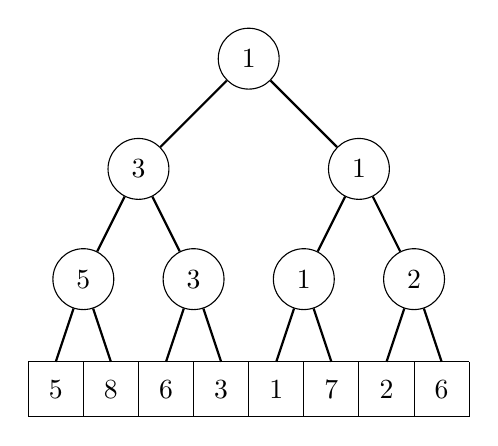
\begin{tikzpicture}[scale=0.7]
\draw (0,0) grid (8,1);

\node[anchor=center] at (0.5, 0.5) {5};
\node[anchor=center] at (1.5, 0.5) {8};
\node[anchor=center] at (2.5, 0.5) {6};
\node[anchor=center] at (3.5, 0.5) {3};
\node[anchor=center] at (4.5, 0.5) {1};
\node[anchor=center] at (5.5, 0.5) {7};
\node[anchor=center] at (6.5, 0.5) {2};
\node[anchor=center] at (7.5, 0.5) {6};

\node[draw, circle,minimum size=22pt] (a) at (1,2.5) {5};
\path[draw,thick,-] (a) -- (0.5,1);
\path[draw,thick,-] (a) -- (1.5,1);
\node[draw, circle,minimum size=22pt] (b) at (3,2.5) {3};
\path[draw,thick,-] (b) -- (2.5,1);
\path[draw,thick,-] (b) -- (3.5,1);
\node[draw, circle,minimum size=22pt] (c) at (5,2.5) {1};
\path[draw,thick,-] (c) -- (4.5,1);
\path[draw,thick,-] (c) -- (5.5,1);
\node[draw, circle,minimum size=22pt] (d) at (7,2.5) {2};
\path[draw,thick,-] (d) -- (6.5,1);
\path[draw,thick,-] (d) -- (7.5,1);

\node[draw, circle,minimum size=22pt] (i) at (2,4.5) {3};
\path[draw,thick,-] (i) -- (a);
\path[draw,thick,-] (i) -- (b);
\node[draw, circle,minimum size=22pt] (j) at (6,4.5) {1};
\path[draw,thick,-] (j) -- (c);
\path[draw,thick,-] (j) -- (d);

\node[draw, circle,minimum size=22pt] (m) at (4,6.5) {1};
\path[draw,thick,-] (m) -- (i);
\path[draw,thick,-] (m) -- (j);
\end{tikzpicture}
\end{center}
\end{samepage}

Tässä segmenttipuussa jokainen puun solmu kertoo,
mikä on pienin luku sen alapuolella olevassa
taulukon osassa.
Segmenttipuun ylin luku on pienin luku
koko taulukon alueella.
Puun toteutus on samanlainen kuin summan laskemisessa,
mutta joka kohdassa pitää laskea summan sijasta
lukujen minimi.

\subsubsection{Binäärihaku puussa}

Segmenttipuun sisältämää tietoa voi käyttää
binäärihaun kaltaisesti aloittamalla
haun puun huipulta.
Näin on mahdollista selvittää esimerkiksi
minimisegmenttipuusta $O(\log n)$-ajassa,
missä kohdassa on taulukon pienin luku.

Esimerkiksi seuraavassa puussa pienin
alkio on 1, jonka sijainti löytyy
kulkemalla puussa huipulta alaspäin:

\begin{center}
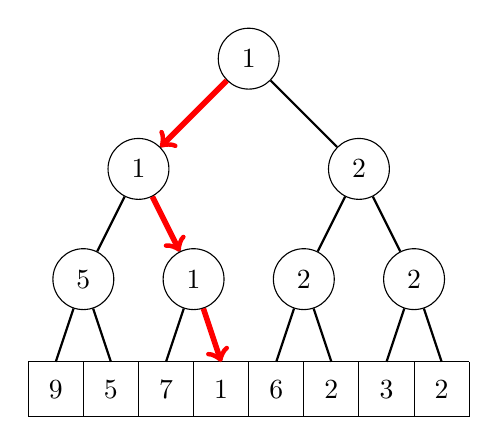
\begin{tikzpicture}[scale=0.7]
\draw (8,0) grid (16,1);

\node[anchor=center] at (8.5, 0.5) {9};
\node[anchor=center] at (9.5, 0.5) {5};
\node[anchor=center] at (10.5, 0.5) {7};
\node[anchor=center] at (11.5, 0.5) {1};
\node[anchor=center] at (12.5, 0.5) {6};
\node[anchor=center] at (13.5, 0.5) {2};
\node[anchor=center] at (14.5, 0.5) {3};
\node[anchor=center] at (15.5, 0.5) {2};

%\node[anchor=center] at (1,2.5) {13};

\node[draw, circle,minimum size=22pt] (e) at (9,2.5) {5};
\path[draw,thick,-] (e) -- (8.5,1);
\path[draw,thick,-] (e) -- (9.5,1);
\node[draw, circle,minimum size=22pt] (f) at (11,2.5) {1};
\path[draw,thick,-] (f) -- (10.5,1);
\path[draw,thick,-] (f) -- (11.5,1);
\node[draw, circle,minimum size=22pt] (g) at (13,2.5) {2};
\path[draw,thick,-] (g) -- (12.5,1);
\path[draw,thick,-] (g) -- (13.5,1);
\node[draw, circle,minimum size=22pt] (h) at (15,2.5) {2};
\path[draw,thick,-] (h) -- (14.5,1);
\path[draw,thick,-] (h) -- (15.5,1);

\node[draw, circle,minimum size=22pt] (k) at (10,4.5) {1};
\path[draw,thick,-] (k) -- (e);
\path[draw,thick,-] (k) -- (f);
\node[draw, circle,minimum size=22pt] (l) at (14,4.5) {2};
\path[draw,thick,-] (l) -- (g);
\path[draw,thick,-] (l) -- (h);

\node[draw, circle,minimum size=22pt] (n) at (12,6.5) {1};
\path[draw,thick,-] (n) -- (k);
\path[draw,thick,-] (n) -- (l);


\path[draw=red,thick,->,line width=2pt] (n) -- (k);
\path[draw=red,thick,->,line width=2pt] (k) -- (f);
\path[draw=red,thick,->,line width=2pt] (f) -- (11.5,1);
\end{tikzpicture}
\end{center}

\section{Lisätekniikoita}

\subsubsection{Indeksien pakkaus}

Taulukon päälle rakennettujen tietorakenteiden
rajoituksena on, että alkiot on indeksoitu
kokonaisluvuin $1,2,3,$ jne.
Tästä seuraa ongelmia,
jos tarvittavat indeksit ovat suuria.
Esimerkiksi indeksin $10^9$ käyttäminen
vaatisi, että taulukossa olisi $10^9$ alkiota,
mikä ei ole realistista.

\index{indeksien pakkaus@indeksien pakkaus}

Tätä rajoitusta on kuitenkin mahdollista
kiertää usein käyttämällä \key{indeksien pakkausta},
jolloin indeksit jaetaan
uudestaan niin, että ne ovat
kokonaisluvut $1,2,3,$ jne.
Tämä on mahdollista silloin, kun kaikki
algoritmin aikana tarvittavat indeksit
ovat tiedossa algoritmin alussa.

Ideana on korvata jokainen alkuperäinen
indeksi $x$ indeksillä $p(x)$,
missä $p$ jakaa indeksit uudestaan.
Vaatimuksena on, että indeksien järjestys
ei muutu, eli jos $a<b$, niin $p(a)<p(b)$,
minkä ansiosta kyselyitä voi tehdä
melko tavallisesti indeksien pakkauksesta huolimatta.

Esimerkiksi jos alkuperäiset indeksit ovat
$555$, $10^9$ ja $8$, ne muuttuvat näin:

\[
\begin{array}{lcl}
p(8) & = & 1 \\
p(555) & = & 2 \\
p(10^9) & = & 3 \\
\end{array}
\]

\subsubsection{Välin muuttaminen}

Tähän asti olemme toteuttaneet tietorakenteita,
joissa voi tehdä tehokkaasti välikyselyitä
ja muuttaa yksittäisiä taulukon arvoja.
Tarkastellaan lopuksi käänteistä tilannetta,
jossa pitääkin muuttaa välejä ja 
kysellä yksittäisiä arvoja.
Keskitymme operaatioon,
joka kasvattaa kaikkia välin $[a,b]$ arvoja $x$:llä.

Yllättävää kyllä,
voimme käyttää tämän luvun tietorakenteita myös tässä tilanteessa.
Tämä vaatii, että muutamme taulukkoa niin,
että jokainen taulukon arvo kertoo \textit{muutoksen}
edelliseen arvoon nähden.
Esimerkiksi taulukosta

\begin{center}
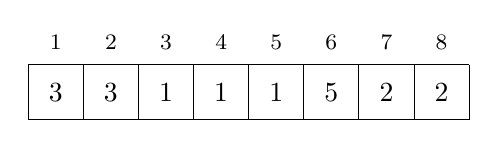
\begin{tikzpicture}[scale=0.7]
\draw (0,0) grid (8,1);

\node at (0.5,0.5) {$3$};
\node at (1.5,0.5) {$3$};
\node at (2.5,0.5) {$1$};
\node at (3.5,0.5) {$1$};
\node at (4.5,0.5) {$1$};
\node at (5.5,0.5) {$5$};
\node at (6.5,0.5) {$2$};
\node at (7.5,0.5) {$2$};


\footnotesize
\node at (0.5,1.4) {$1$};
\node at (1.5,1.4) {$2$};
\node at (2.5,1.4) {$3$};
\node at (3.5,1.4) {$4$};
\node at (4.5,1.4) {$5$};
\node at (5.5,1.4) {$6$};
\node at (6.5,1.4) {$7$};
\node at (7.5,1.4) {$8$};
\end{tikzpicture}
\end{center}
tulee seuraava:
\begin{center}
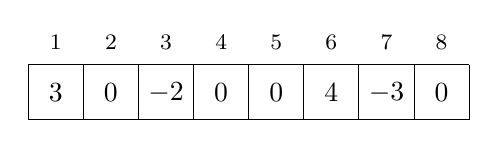
\begin{tikzpicture}[scale=0.7]
\draw (0,0) grid (8,1);

\node at (0.5,0.5) {$3$};
\node at (1.5,0.5) {$0$};
\node at (2.5,0.5) {$-2$};
\node at (3.5,0.5) {$0$};
\node at (4.5,0.5) {$0$};
\node at (5.5,0.5) {$4$};
\node at (6.5,0.5) {$-3$};
\node at (7.5,0.5) {$0$};


\footnotesize
\node at (0.5,1.4) {$1$};
\node at (1.5,1.4) {$2$};
\node at (2.5,1.4) {$3$};
\node at (3.5,1.4) {$4$};
\node at (4.5,1.4) {$5$};
\node at (5.5,1.4) {$6$};
\node at (6.5,1.4) {$7$};
\node at (7.5,1.4) {$8$};
\end{tikzpicture}
\end{center}

Minkä tahansa vanhan arvon saa uudesta taulukosta
laskemalla summan taulukon alusta kyseiseen kohtaan asti.
Esimerkiksi kohdan 6 vanha arvo 5 saadaan
summana $3-2+4=5$.

Uuden tallennustavan etuna on,
että välin muuttamiseen riittää muuttaa
kahta taulukon kohtaa.
Esimerkiksi jos välille $2 \ldots 5$
lisätään luku 5,
taulukon kohtaan 2 lisätään 5
ja taulukon kohdasta 6 poistetaan 5.
Tulos on tässä:

\begin{center}
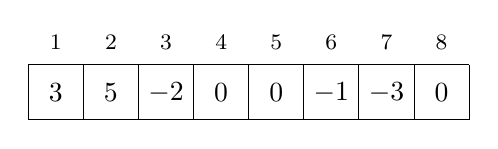
\begin{tikzpicture}[scale=0.7]
\draw (0,0) grid (8,1);

\node at (0.5,0.5) {$3$};
\node at (1.5,0.5) {$5$};
\node at (2.5,0.5) {$-2$};
\node at (3.5,0.5) {$0$};
\node at (4.5,0.5) {$0$};
\node at (5.5,0.5) {$-1$};
\node at (6.5,0.5) {$-3$};
\node at (7.5,0.5) {$0$};

\footnotesize
\node at (0.5,1.4) {$1$};
\node at (1.5,1.4) {$2$};
\node at (2.5,1.4) {$3$};
\node at (3.5,1.4) {$4$};
\node at (4.5,1.4) {$5$};
\node at (5.5,1.4) {$6$};
\node at (6.5,1.4) {$7$};
\node at (7.5,1.4) {$8$};
\end{tikzpicture}
\end{center}

Yleisemmin kun taulukon välille $a \ldots b$
lisätään $x$, taulukon kohtaan $a$
lisätään $x$ ja taulukon kohdasta $b+1$
vähennetään $x$.
Tarvittavat operaatiot 
ovat summan laskeminen
taulukon alusta tiettyyn kohtaan
sekä yksittäisen alkion muuttaminen,
joten voimme käyttää tuttuja menetelmiä tässäkin tilanteessa.

Hankalampi tilanne on, jos samaan aikaan pitää pystyä
sekä kysymään tietoa väleiltä että muuttamaan välejä.
Myöhemmin luvussa 28 tulemme näkemään,
että tämäkin on mahdollista.



